\documentclass[final,5p,times,twocolumn,authoryear]{elsarticle}

%% ---------- Maths ----------
\usepackage{amssymb}
\usepackage{amsmath}

%% ---------- Colours and links (xcolor before hyperref) ----------
\usepackage{xcolor}
\definecolor{myteal}{RGB}{0,128,128}
\usepackage[colorlinks]{hyperref}
\AtBeginDocument{%
  \hypersetup{
    citecolor=myteal,
    linkcolor=myteal,
    urlcolor=myteal
  }%
}

%% ---------- URL line breaking ----------
\usepackage{url}

%% ---------- Tables ----------
\usepackage{tabularx}
\usepackage{booktabs}
\usepackage{array}

%% Flexible column, left aligned, automatic line wrapping
\newcolumntype{Y}{>{\raggedright\arraybackslash}X}
%% Weighted flexible column, e.g. Z{0.8} is 0.8x the default share
\newcolumntype{Z}[1]{>{\raggedright\arraybackslash\hsize=#1\hsize}X}

%% ---------- Float behaviour: pack figures with text ----------
%% Allow generous top floats so pages combine figures and prose
%% rather than isolating one figure per page.
\setcounter{topnumber}{3}
\setcounter{dbltopnumber}{3}
\setcounter{totalnumber}{5}
\renewcommand{\topfraction}{0.92}
\renewcommand{\dbltopfraction}{0.92}
\renewcommand{\textfraction}{0.06}
\renewcommand{\floatpagefraction}{0.85}
\renewcommand{\dblfloatpagefraction}{0.85}
%% Tighten space between floats and text
\setlength{\textfloatsep}{10pt plus 2pt minus 2pt}
\setlength{\dbltextfloatsep}{10pt plus 2pt minus 2pt}
\setlength{\floatsep}{8pt plus 2pt minus 2pt}
\setlength{\dblfloatsep}{8pt plus 2pt minus 2pt}

%% ---------- Journal ----------
%% ---------- Tighter vertical margins ----------
\usepackage{geometry}
\geometry{top=18mm, bottom=18mm}

\journal{Journal of Transport Geography}

\begin{document}

%TC:ignore
\onecolumn
\thispagestyle{empty}

\vspace*{2cm} 
\noindent\textbf{Note:} This paper is prepared for submission to the
\textit{Journal of Transport Geography} (JTG). JTG is the leading venue for
research on the spatial dimensions of transport systems and their
consequences for accessibility, and regularly publishes work on cycling
network analysis, Level of Traffic Stress methodology, and infrastructure
data quality assessment. The paper's combination of spatial network methods
with a nationally scoped design-standard classification aligns directly with
the journal's scope.

\vspace{0.4cm}

\noindent The manuscript is typeset using the official Elsevier \LaTeX\ template in two-column layout. Although JTG does
not require a specific column format for submission, the two-column
presentation was chosen because the Results section contains a large number
of full-width figures and tables; the narrower text columns allow these
floats to be interleaved more closely with their surrounding discussion,
improving readability and reducing the number of pages that separate a figure
from the text that references it.

\vspace{\fill}

\begin{center}
{\large\bfseries MRes Publication}\\[1.8cm]

Candidate: Zhengpei Xu\\[0.3cm]
Student Number: 25034404\\[1.2cm]

Journal: \textit{Journal of Transport Geography}\\[1.2cm]

Word Count for Main Body: 5,538\\[0.2cm]
Word Count including Headers and Captions: 5,947\\[1.2cm]

Submission Date: August 2026\\[0.2cm]
Module Name: MRes Dissertation\\[0.2cm]
Module ID: CASA0004\\[0.2cm]
Supervisor: Prof Duncan Smith
\end{center}

\vspace{\fill}

\clearpage
\twocolumn
%TC:endignore

\begin{frontmatter}

\title{Adapting Level of Traffic Stress for England: A Network-Scale Cycling
Infrastructure Assessment in the West Midlands}

\author[CASA]{Zhengpei Xu}

\affiliation[CASA]{organization={Centre for Advanced Spatial Analysis (CASA), University College London},
            city={London},
            postcode={W1T 4TJ},
            country={United Kingdom}}

%TC:ignore
\begin{abstract}
England's most comprehensive national design standard for cycling infrastructure, Local Transport Note 1/20 (LTN~1/20), is anchored in the principle that cycling should be accessible to everyone. Its evaluation instruments, however, were conceived for scheme-level auditing and cannot assess whether compliant schemes cohere into a network navigable at tolerable stress levels for cyclists. This paper develops a Level of Traffic Stress (LTS) classification derived entirely from LTN~1/20's design criteria, the first calibrated to English design standards, and operationalises it using the newly released Ordnance Survey National Geographic Database (OS~NGD) Cycle Lane data. The classification incorporates directed junction assessment grounded in LTN~1/20's Junction Assessment Tool, with bearing-based conflict detection and roundabout-specific criteria absent from prior LTS implementations. Applied to the West Midlands, the English region with the highest share of private motorised trips and a cycling mode share of 0.9\%, the framework shows that abundant low-stress length does not constitute a usable network. Low-stress segments comprise over three-quarters of network length yet fragment into thousands of disconnected components: junction stress concentrates where residential clusters must cross arterial roads, and roundabouts act as high-stress and dangerous barriers. Only 4.1\% of residents can reach their nearest school at conditions suitable for children, and only 13.0\% of short-distance commuting flow is connected at stress levels tolerable to mainstream adults, with connected pairs facing a median detour of 1.76 times the shortest path. The first independent comparison with OpenStreetMap further establishes the strengths and limitations of the OS~NGD Cycle Lane dataset. With nationally consistent thresholds and data, the framework enables systematic, comparable evaluation of the cycling network for any English region against established statutory standards.
\end{abstract}

\begin{keyword}
Cycling infrastructure \sep Level of Traffic Stress \sep Network connectivity \sep Bicycle network \sep Design standards \sep Accessibility
\end{keyword}
%TC:endignore

\end{frontmatter}

%% ============================================================
\section{Introduction}
\label{sec:intro}

Cycling is widely recognised as a sustainable mode of urban transport, offering co-benefits across public health, air quality, carbon reduction and potential congestion alleviation \citep{who2022, eu2024, ipcc2023}. Central to realising these benefits is high-quality, connected cycling infrastructure, which is consistently associated with higher cycling participation \citep{hull2014, buehler2016, molenberg2019}. Reflecting this evidence, the UK Department for Transport published Local Transport Note 1/20, \textit{Cycle infrastructure design} (LTN~1/20), in July 2020, establishing the most comprehensive national standards for cycling infrastructure design and assessment applicable to England and Northern Ireland to date \citep{departmentfortransport2020a}. Its evaluation tools, the Cycling Level of Service (CLoS) and the Junction Assessment Tool (JAT), give practitioners a rigorous means of appraising individual schemes through structured manual auditing. What they do not address is the network-level question: whether compliant segments cohere into a connected whole. Cycling connectivity is a property of whole journeys rather than individual schemes, and a single high-stress link or junction can render an otherwise compliant route unusable for the very cyclists the guidance seeks to serve. A data-driven, network-level methodology is therefore needed to evaluate cycling infrastructure quality across a city or region using standard open and mapping agency data.

The Level of Traffic Stress (LTS) framework offers such an approach, classifying road segments and junctions by the population group willing to tolerate their traffic conditions, from LTS~1, suitable for children, to LTS~4, tolerable only to the most confident riders \citep{mekuria2012a}. Because each stress level maps onto a population group, the classification links infrastructure quality directly to mode shift potential: expanding the network usable at lower stress thresholds is what brings the broader population into cycling. LTS-based analysis has since become a leading approach in cycling connectivity and equity research \citep{louro2026}. Yet most published LTS criteria were calibrated to North American road design conventions, and applications to British cities have relied on simplified adaptations of these criteria rather than national design guidance \citep{cervero2019, jeong2025}. No LTS classification grounded in UK design standards has been developed systematically.

The recent release of the Ordnance Survey National Geographic Database (OS~NGD) Cycle Lane feature collection provides, for the first time, a nationally consistent and authoritative cycling infrastructure dataset with facility descriptions aligned to LTN~1/20 terminology, recording cycle lane width, direction of travel and infrastructure type \citep{ordnancesurvey2026e}. The wider OS~NGD Transport Theme adds network geometry together with attributes directly relevant to stress classification, including carriageway width, legal access designation and probe-derived vehicle speeds. Together, a statutory design standard and a nationally consistent dataset enable cycling networks across England to be evaluated against a single national benchmark.

This paper develops a directed LTS classification derived from LTN~1/20 design criteria, operationalises it on OS~NGD Transport data, and applies it to the West Midlands. Among English regions, the West Midlands combines the highest share of private motorised trips with a cycling mode share of only 0.9\% \citep{westmidlandscombinedauthority2024}, yet its transport authority has committed to delivering a 500-mile network of low-stress cycle routes \citep{westmidlandscombinedauthority2020}; the distance between this ambition and current network conditions is precisely what a standards-based classification is designed to measure. The study, conducted in collaboration with Transport for West Midlands, makes two contributions: the first LTS framework calibrated systematically to English design standards, incorporating directed junction assessment and roundabout-specific criteria; and the first independent assessment of the OS~NGD Cycle Lane dataset. The classified network is used to evaluate connectivity against LTN~1/20's own principle of ``cycling for all'', examining the spatial distribution of low-stress provision, its cohesion into connected components, the reach available to residents from where they live, and the share of school travel and commuting demand the network can carry at each stress threshold.

%% ============================================================
\section{Background}
\label{sec:background}

\subsection{From Perceived Safety to Network Connectivity}
\label{sec:perceived-safety}

The positive association between infrastructure provision and cycling participation is generally explained through safety, and specifically its subjective dimension: it is perceived safety, rather than the volume of recorded crash incidents, that most directly shapes the decision to cycle, particularly for prospective and occasional riders \citep{chaurand2013, sanders2015, manton2016}. Early work characterised the discomfort imposed by the speed, volume and proximity of motor traffic as a graded property of the road environment that can be inferred from a road's physical and operational characteristics \citep{sorton1994, landis1997, harkey1998}, making the deterrent effect of traffic legible in terms of design variables that infrastructure can be built to modify. Tolerance of this stress is not uniform across the population: groups under-represented among cyclists, women in particular, express stronger preferences for separation from motor traffic, with converging evidence for older adults and those cycling with children \citep{aldred2017}. The latent demand that infrastructure investment seeks to convert is therefore concentrated among the ``interested but concerned'', individuals who would cycle if protected from stressful traffic and who represent the largest and most winnable constituency for mode shift \citep{geller2009, dill2013}. Route choice evidence further shows that cyclists accept meaningful detours to avoid stressful links and crossings, evaluating routes as integrated wholes rather than collections of independent facilities \citep{broach2012, park2019, berghoefer2023}; where no acceptable alternative exists, a single hostile link or crossing renders an otherwise suitable route unacceptable \citep{mekuria2012a, furth2018}. The infrastructure quality relevant to the stress-averse majority is thus a property of connected networks rather than of individual facilities, and its assessment requires criteria referenced to the populations expected to use them, applied to whole journeys rather than isolated schemes.

\subsection{LTN~1/20: Design Standards for Cycling Infrastructure in England}
\label{sec:ltn120-limits}

Published alongside the \textit{Gear Change} white paper, which set the ambition that half of urban journeys be cycled or walked by 2030 \citep{departmentfortransport2020}, LTN~1/20 establishes as first principle that cycle infrastructure should be accessible to everyone ``from 8 to 80 and beyond'' \citep{departmentfortransport2020a}. Its evaluation framework, organised around five design principles derived from Dutch practice \citep{crow2016}, comprises two instruments: the Cycling Level of Service (CLoS), which scores 25 link-level subcriteria from 0 to 2 with designated critical failures, and the Junction Assessment Tool (JAT), whose three scoring tiers are explicitly anchored to distinct user populations. With the establishment of Active Travel England as national inspectorate in 2022, these instruments became binding: only schemes achieving a CLoS score of at least 70\%, with no critical failures and no red-scored JAT movements, are generally eligible for Active Travel Fund allocations, effectively transforming LTN~1/20 from advisory guidance into a quality threshold for publicly funded infrastructure.

Three structural limitations constrain these tools as a framework for network-wide assessment. First, both are scheme-level audit instruments requiring on-site evaluation by trained assessors, an approach that cannot feasibly scale to all cyclable links across an urban network and that risks inconsistency where subcriteria demand qualitative judgement \citep{hancock2024}. Second, the CLoS mixes stress-determinant factors that implicitly delineate population acceptability, such as motor traffic speed, volume and segregation, with experience-quality factors that do not, such as wayfinding and cycle parking; its additive scoring is inherently compensatory \citep{pais2022, wang2022}, so a link may satisfy the 70\% threshold through the latter while falling short on stress conditions that would deter most potential cyclists. Third, although the CLoS includes coherence subcriteria, these assess attributes of individual links and cannot answer whether a cyclist can complete a journey from origin to destination entirely within tolerable traffic conditions, despite end-to-end low-stress connectivity being the most fundamental determinant of a network's capacity to attract the wider population \citep{mekuria2012a, wang2016, lowry2017}.

\subsection{Level of Traffic Stress and the Gap in English Practice}
\label{sec:lts-gap}

Where LTN~1/20 operationalises ``cycling for all'' through a broad composite of design criteria, the LTS framework makes population acceptability the sole organising principle of classification. Adapting \citeauthor{geller2009}'s (\citeyear{geller2009}) cyclist typology, validated by \citet{dill2013}, \citet{mekuria2012a} defined four levels each anchored to a distinct population group, from children (LTS~1) through the mainstream ``interested but concerned'' adult majority (LTS~2) to progressively smaller and more confident groups of experienced cyclists (LTS~3 and~4). Classification draws on the road characteristics most directly associated with cycling stress, notably motor traffic speed, facility type and width, and crossing conditions, and follows a non-compensatory rule: a segment's LTS is determined by its worst-performing attribute. The framework's connectivity measures, quantifying the share of origin--destination pairs connected at each stress threshold, have been widely adopted for cumulative accessibility, transport equity and investment prioritisation analysis \citep{furth2016, lowry2017, tucker2018, schon2024}, making LTS the dominant approach in cycling accessibility research \citep{louro2026}.

Two limitations constrain existing implementations in the UK context. First, all published criteria were calibrated to North American design conventions, speed regimes and infrastructure types; applications to British cities \citep{cervero2019, jeong2025} relied on simplified adaptations rather than national design guidance. Second, progressive simplification of the original criteria for network-scale application has produced considerable methodological divergence, with \citet{harvey2024} finding substantial disagreement across seven LTS methods applied to the same cities. Rather than adapting any single North American variant, this study therefore grounds the classification in LTN~1/20, a single national standard that provides both the threshold structure and the population-acceptability logic needed to anchor LTS to English conditions. This paper aims to, first, operationalise LTN 1/20's design criteria into a directed, network-scale LTS classification, including junction and roundabout assessment, using OS NGD Transport data; and second, evaluate the extent to which the West Midlands network delivers the connected, low-stress conditions that "cycling for all" requires, for the population groups the standard identifies.

%% ============================================================
\section{Study area and data}
\label{sec:study-area}

The West Midlands metropolitan region comprises the seven boroughs of Birmingham, Coventry, Dudley, Sandwell, Solihull, Walsall and Wolverhampton, and with over 3~million residents is Britain's second most populated conurbation \citep{officefornationalstatistics2025}. The region is polycentric, with Birmingham as the dominant core surrounded by densely populated centres including Wolverhampton, Coventry and the Black Country towns, while southern and eastern Solihull and the fringes of Walsall and Birmingham are predominantly rural (Fig.~\ref{fig:study-area}). A century of automobile manufacturing and post-war road building, including Britain's first urban motorway \citep{gunn2018}, entrenched car-oriented mobility: the wider region records the highest share of private motorised trips among English regions, at 69\% in 2024 \citep{departmentfortransport2025}, while cycling accounts for approximately 0.9\% of trips despite 41\% of car journeys being under two miles \citep{westmidlandscombinedauthority2019, westmidlandscombinedauthority2024}. Transport for West Midlands has responded with the Starley Network, a planned 500-mile network of traffic-free or physically separated cycle routes aligned with LTN~1/20 \citep{westmidlandscombinedauthority2020}, yet the gap between this policy ambition and measurable network conditions remains unquantified.

\begin{figure*}[!t]
\centering

\includegraphics[width=0.82\textwidth]{figure/study_area_map.png}
\caption{The West Midlands metropolitan region: population density by LSOA (Census 2021).}
\label{fig:study-area}
\end{figure*}

The analysis draws on four principal sources (Table~\ref{tab:datasets}). OS~NGD Transport provides network geometry, road classification, carriageway and cycle lane width, legal access designation, junction form and probe-derived average speeds; its Cycle Lane feature collection achieved full national coverage in March 2026 \citep{ordnancesurvey2026e}, making this among the first studies to incorporate authoritative national cycling infrastructure data into a network-level assessment. Department for Transport road traffic counts supply observed AADT volumes and training data for minor road volume estimation. OpenStreetMap (OSM) contributes cycling geometries for Path Link cross-validation, traffic signal locations for junction classification, and school locations for accessibility analysis. Census data from the Office for National Statistics provide MSOA-level commuting flows and LSOA-level population and boundaries.

\begin{table*}[!t]
\centering
\caption{Datasets used in the analysis.}
\label{tab:datasets}
\small
\begin{tabularx}{\textwidth}{Z{0.85} Z{0.6} Z{1.9} Z{0.65}}
\toprule
Dataset & Provider & Key variables & Spatial unit \\
\midrule
Road Links & OS NGD & Geometry, classification, description, width & Edge \\
Path Links & OS NGD & Geometry, cycle lane presence & Edge \\
Highway Dedication & OS NGD & Legal access designation & Edge \\
Cycle Lane & OS NGD & Facility type, width, placement side & Edge \\
Average Speed (RAMI) & OS NGD & Mean vehicle speeds by time period & Edge \\
Road Node & OS NGD & Node form, geometry, description & Node \\
Path Node & OS NGD & Node geometry & Node \\
Road Traffic Counts & DfT & Annual Average Daily Traffic (AADT) by vehicle type & Count point \\
Cycling Network & OSM & Highway and cycleway tags & Way \\
Traffic Signals & OSM & Signal node locations & Node \\
Schools & OSM & Location & Point \\
Commuting Flows & ONS & OD pairs within 8~km (Census 2011) & MSOA \\
Population & ONS & Resident population (Census 2021) & LSOA \\
Boundaries & ONS & LSOA/MSOA polygons & Polygon \\
\bottomrule
\end{tabularx}
\end{table*}

%% ============================================================
\section{Methodology}
\label{sec:methodology}

The framework proceeds in two stages: constructing the directed, stress-classified network by extracting cyclable segments, assigning link-level LTS and propagating junction stress under LTN~1/20's criteria (Sections~\ref{sec:extraction} to~\ref{sec:junction-lts}), then evaluating connectivity against the ``cycling for all'' principle through density, fragmentation, reach and origin--destination analyses (Section~\ref{sec:connectivity}). 

\subsection{Cyclable Network Extraction and Facility Classification}
\label{sec:extraction}

Cyclable infrastructure appears in two OS~NGD feature collections: Road Links \citep{ordnancesurvey2026a}, representing the carriageway network, and Path Links, representing routes topologically independent from it \citep{ordnancesurvey2026b}. Legal cyclability is established through the Highway Dedication collection, five of whose designation types permit cycling under UK highway law, while `Motorway' and `Pedestrian Way Or Footpath' are excluded as non-cyclable (Table~\ref{tab:dedication}). For Road Links, where dedication is absent or recorded as unknown, a fallback classification retains segments whose physical description indicates a carriageway type. This yields 212,551 cyclable Road Links (97.8\%), of which 84.2\% are identified through Highway Dedication and 15.8\% through the fallback. For Path Links, Highway Dedication identifies only 10.1\% of cyclable paths and no schema attribute provides a direct cyclability indicator. Two further layers are therefore applied: the `presenceofcyclelane' attribute contributes another 1.0\%, and spatial cross-validation against the OpenStreetMap cycling network within a 5~m nearest-neighbour join recovers a further 40,035 paths. Together these yield 45,023 cyclable Path Links (40.3\% of the collection). Paths with explicitly non-cyclable dedications are excluded at all layers. Each segment is then expanded into directed edges, with cycle lane records joined only to the edge whose travel direction matches the lane's placement side, capturing the asymmetric distribution of infrastructure and avoiding overestimation of provision.

\begin{table*}[!t]
\centering
\caption{Cyclability by Highway Dedication type. The eighth type, `No Dedication Or Dedication Unknown', is addressed through the description-based fallback for Road Links.}
\label{tab:dedication}
\small
\begin{tabularx}{\textwidth}{Z{1.0} Z{0.45} Z{1.55}}
\toprule
Highway Dedication & Cyclable? & Legal basis \\
\midrule
All Vehicles & Yes & Cycling permitted on public roads by default \\
Cycle Track or Cycle Way & Yes & Cycle Tracks Act 1984 \\
Bridleway & Yes & Countryside Act 1968, s.30 \\
Restricted Byway & Yes & Countryside and Rights of Way Act 2000 \\
Byway Open to All Traffic & Yes & Wildlife and Countryside Act 1981, s.66(1) \\
Motorway & No & Motorways Traffic (England and Wales) Regulations 1982 \\
Pedestrian Way or Footpath & No & No public right of way for cycling (cf.\ Highways Act 1835, s.72) \\
\bottomrule
\end{tabularx}
\end{table*}

Each directed segment is classified into one of eight facility types derived from LTN~1/20's design hierarchy (Table~\ref{tab:facility}), using the OS~NGD Cycle Lane dataset, whose type definitions align to LTN~1/20 and which records dedicated infrastructure as separate features referencing their parent Road Link \citep{ordnancesurvey2026d}. Where multiple cycle lane records exist for a link, the more protective facility governs; links without a matching record, or recorded as `Unknown Type Of Cycle Track Or Lane', default to Mixed Traffic. All cyclable Path Links are classified as Off-Road, as they are topologically independent from the road network and carry no motor traffic speed or volume attributes. Road Links and Path Links are then merged into a single unified directed network.

\begin{table*}[!t]
\centering
\caption{Facility type classification. Off-Road paths may in practice function as shared-use routes or kerbed tracks; this does not affect the LTS classification, as all such facilities are fully separated from motor traffic.}
\label{tab:facility}
\small
\begin{tabularx}{\textwidth}{Z{0.75} Z{0.6} Z{1.65}}
\toprule
Facility type & OS NGD source & Classification feature \\
\midrule
Off-Road & Path Link & Cyclable Path Links \\
Shared Use & Cycle Lane & `Unsegregated Shared Use Cycle Facility' / `Segregated Shared Use Cycle Track' \\
Fully Kerbed Cycle Track & Cycle Lane & `Fully Segregated Cycle Track' \\
Stepped Cycle Track & Cycle Lane & `Stepped Cycle Track Along Road' \\
Light Segregation & Cycle Lane & `Lightly Segregated Cycle Lane On Road' \\
Mandatory Cycle Lane & Cycle Lane & `Mandatory Cycle Lane On Road' \\
Advisory Cycle Lane & Cycle Lane & `Advisory Cycle Lane On Road' \\
Mixed Traffic & Road Link (main) & `Unknown Type Of Cycle Track Or Lane' or no matching Cycle Lane record \\
\bottomrule
\end{tabularx}
\end{table*}

\subsection{Link-level LTS Classification}
\label{sec:link-lts}

The link-level classification adapts the \citet{mekuria2012a} framework by replacing its North American thresholds with those of LTN~1/20. Although the CLoS assessment as a whole allows a high score on one criterion to offset a low score on another, its core Safety subcriteria addressing motor traffic speed (Criterion~10), volume (Criterion~11) and segregation provision and carriageway width (Criterion~12) are themselves non-compensatory stress determinants built on CROW-derived logic \citep{crow2016}, directly consistent with the LTS framework. This graduated logic is mapped onto the four LTS levels (Table~\ref{tab:link-lts}): conditions suitable for all users including children (LTS~1), most adults (LTS~2), confident cyclists (LTS~3), and conditions triggering a critical safety failure under LTN~1/20 criteria (LTS~4). Where multiple criteria apply, the worst-performing criterion governs.

\begin{table*}[!t]
\centering
\caption{Link-level LTS classification criteria. (1)~The overall LTS is determined by the worst-performing criterion (non-compensatory). (2)~Thresholds derive from the CLoS Safety subcriteria (Criteria 9--12, 15) in LTN~1/20 Appendix~A, supplemented by the speed--volume--facility matrix in Figure~4.1. (3)~AADT is used as a proxy for the PCU thresholds in Criterion~11; HGV composition thresholds could not be applied due to the absence of network-wide composition data. (4)~Rural exception: mixed traffic segments with $V_{85} \leq 30$~mph and AADT $\leq 1{,}000$ are classified LTS~1, following LTN~1/20 Figure~4.1 Note~3.}
\label{tab:link-lts}
\footnotesize
\begin{tabularx}{\textwidth}{Z{0.85} Z{1.0} Z{1.0} Z{1.05} Z{1.1}}
\toprule
Facility type & LTS 1 & LTS 2 & LTS 3 & LTS 4 \\
\midrule
Off-Road & All conditions & -- & -- & -- \\
Shared Use & All conditions & -- & -- & -- \\
Fully Kerbed Cycle Track & All conditions & -- & -- & -- \\
Stepped cycle track & $V_{85} \leq 30$ mph & $V_{85}$ 30--37 mph & $\geq 37$ mph & -- \\
Light segregation & $V_{85} \leq 30$ mph & $V_{85}$ 30--37 mph & $\geq 37$ mph & -- \\
Mandatory cycle lane & Width $\geq 1.8$ m, $V_{85} \leq 20$ mph, AADT $\leq 5{,}000$ & Width $\geq 1.8$ m, $V_{85}$ 20--30 mph, AADT $\leq 5{,}000$ & Width $< 1.8$ m; or $V_{85}$ 30--37 mph; or AADT 5,000--10,000 & $V_{85} \geq 37$ mph; or AADT $\geq 10{,}000$ \\
Advisory cycle lane & Width $\geq 1.8$ m, $V_{85} \leq 20$ mph, AADT $\leq 5{,}000$ & Width $\geq 1.8$ m, $V_{85}$ 20--30 mph, AADT $\leq 5{,}000$ & Width $< 1.8$ m; or $V_{85}$ 30--37 mph; or AADT 5,000--10,000 & $V_{85} \geq 37$ mph; or AADT $\geq 10{,}000$ \\
Mixed traffic & $V_{85} \leq 20$ mph, AADT $\leq 2{,}500$ & $V_{85}$ 20--30 mph, AADT 2,500--5,000 & $V_{85}$ 30--37 mph; or AADT 5,000--10,000 & $V_{85} \geq 37$ mph; or AADT $\geq 10{,}000$; or nearside lane 3.2--3.9 m and AADT $\geq 5{,}000$ \\
\bottomrule
\end{tabularx}
\end{table*}

Three primary variables drive classification alongside facility type. Width uses the modal cycle lane width, which better captures typical conditions along a segment than the minimum one; for mixed traffic on single carriageways, average road width identifies the critical nearside lane range of 3.2 to 3.9~m associated with elevated close-pass risk, an override triggering LTS~4. Prevailing speed is represented by the estimated 85th percentile speed ($V_{85}$), the measurement basis specified in LTN~1/20 and a more reliable stress measure than official speed limits, from which operating speeds frequently diverge \citep{europeancommission2021, departmentfortransport2025b}. $V_{85}$ is estimated from OS~NGD probe-derived mean speeds by applying a 7/6 multiplier following CA~185 \citep{nationalhighways2019}, which approximates $V_{85}$ as the mean plus one sixth of the mean under a normality assumption. Motor traffic volume, absent from OS~NGD, is taken from DfT AADT count points for major roads and estimated for minor roads following \citet{morley2016}: a Poisson GLM using road network characteristics extracted via pgRouting on the England OSM network as predictors achieves $R^2 = 0.604 \pm 0.019$ and Spearman's $\rho = 0.803 \pm 0.015$ in five-fold cross-validation ($n = 3{,}695$ count points), considered sufficient for the coarse-grained classification task. Values are assigned to OS~NGD links via nearest-network spatial join, with unmatched links imputed by the median AADT of their road classification.

\subsection{Junction LTS Classification}
\label{sec:junction-lts}

The original LTS framework propagated junction stress to approaching minor-street links, but the fine-grained geometric data it requires are unavailable at network scale \citep{furth2018}, driving adoption of the \citet{conveyal2015} method, which propagates the highest segment LTS at each unsignalised vertex to all incident edges without evaluating crossing geometry. Two gaps persist in this widely applied lineage \citep{semler2017, murphy2019}. First, no existing criteria cover roundabouts, despite their prevalence in UK networks and documented cyclist collision risk \citep{daniels2009, aldred2021}. Second, undirected vertex-level propagation assigns elevated stress indiscriminately to all incident edges regardless of legal travel direction, obscuring heterogeneity in crossing conditions.

The JAT evaluates junction suitability by junction form, disaggregated by the cycle movement being assessed. Three variables govern crossing stress: the speed and volume of conflicting motor traffic, determining conflict severity; the number of lanes crossed in one movement, determining exposure duration; and the availability of protection such as a refuge or signals. LTN~1/20's crossing design suitability matrix classifies crossings by these variables into three suitability tiers, which this study maps to LTS~1, LTS~2 and LTS~3--4 respectively (Table~\ref{tab:crossing-lts}). Protection is operationalised in three levels: uncontrolled, traffic island (from the OS~NGD link description ``Traffic Island Link At Junction'') and signalised (from OSM traffic signal tags joined to OS~NGD nodes). Roundabouts are classified directly from the JAT's roundabout-specific criteria, by the maximum AADT, $V_{85}$ and road width of incident links (Table~\ref{tab:roundabout-lts}).

\begin{table*}[!t]
\centering
\caption{Crossing junction LTS classification.}
\label{tab:crossing-lts}
\small
\begin{tabularx}{0.9\textwidth}{l l l Y Y Y}
\toprule
$V_{85}$ (mph) & AADT & Est.\ lanes & Uncontrolled & Traffic island & Signal \\
\midrule
$\geq 37$ & Any & Any & 4 & 4 & 3 \\
30--37 & $> 10{,}000$ & Any & 4 & 4 & 1 \\
30--37 & 6,000--10,000 & $\geq 2$ & 4 & 4 & 1 \\
30--37 & $\leq 6{,}000$ & $\geq 2$ & 3 & 3 & 1 \\
30--37 & $\leq 10{,}000$ & 1 & 2 & 2 & 1 \\
$\leq 30$ & $> 8{,}000$ & $> 2$ & 4 & 3 & 1 \\
$\leq 30$ & $> 8{,}000$ & $\leq 2$ & 3 & 2 & 1 \\
$\leq 30$ & 4,000--8,000 & $\geq 2$ & 2 & 2 & 1 \\
$\leq 30$ & 4,000--8,000 & 1 & 2 & 1 & 1 \\
$\leq 30$ & $\leq 4{,}000$ & $\geq 2$ & 2 & 1 & 1 \\
$\leq 30$ & $\leq 4{,}000$ & 1 & 1 & 1 & 1 \\
\bottomrule
\end{tabularx}
\end{table*}

\begin{table}[!t]
\centering
\caption{Roundabout LTS classification. Signals lower roundabout LTS by one level (min LTS 2), except where a segregated cycle facility is also present.}
\label{tab:roundabout-lts}
\small
\begin{tabularx}{\linewidth}{Y c}
\toprule
Base conditions & LTS \\
\midrule
AADT $> 8{,}000$ and est.\ lanes $\geq 2$; or $V_{85} \geq 37$ mph & 4 \\
AADT $> 8{,}000$ or est.\ lanes $\geq 2$ (but not both) & 3 \\
All other roundabouts (compact/mini, AADT $\leq 8{,}000$) & 2 \\
Segregated cycle facility and traffic signal & 1 \\
\bottomrule
\end{tabularx}
\end{table}


\noindent The classification operates at the (link, junction node) pair level, following the JAT's definition of stress as arising from cycle movements in potential conflict with motor traffic. Conflicting links at each crossing junction are identified via the OS~NGD directionality attribute, retaining only links that a cyclist departing the node could legally enter, and excluding straight-line continuations of the approach link through a bearing-based filter (departure bearing within $180^\circ \pm 30^\circ$, following the orientation criterion in \citealp{mekuria2012a}). The three crossing variables (maximum $V_{85}$, AADT and estimated lane count) are then taken over the remaining conflict links, ensuring they reflect the transverse traffic stream being crossed. For roundabout nodes, where circulatory geometry renders approach-level analysis inapplicable, classification operates at node level across all incident links. In both cases, junction LTS is overlaid onto the segment classification with worst-indicator-wins logic, so that junction stress can only elevate a link's final LTS.

\subsection{Stress-based Connectivity Evaluation}
\label{sec:connectivity}

The following analyses evaluate whether the West Midlands network delivers on the LTN 1/20 "cycling for all" principle by testing connectivity at LTS~1 (children and older adults) and LTS~$\leq 2$ (mainstream adults), with LTS~$\leq 3$ and $\leq 4$ for comparison. Following \citet{viero2025} and \citet{schon2024}, the evaluation proceeds through area-based distribution, network fragmentation, network reach and origin-destination connectivity. Network density is computed at LSOA level as absolute density (km of classified network per km\textsuperscript{2}) and relative density (share of local network at each LTS level), characterising spatial supply independent of connectivity. Fragmentation applies connected component analysis: for each cumulative threshold, edges exceeding it are removed and components identified on the undirected projection, with the largest connected component (LCC), the maximum contiguous network traversable without exceeding the threshold, and its share of sub-network length measuring cohesion. All metrics are computed on the LCC of the full cyclable network, excluding topologically isolated stubs so that measured fragmentation reflects the breaking of connected routes rather than pre-existing disconnection. Network reach is the total length reachable from each LSOA centroid's nearest node within 8~km, the distance within which 70\% of personal trips in England fall \citep{departmentfortransport2025}, computed by directed Dijkstra search on each cumulative subgraph. Two origin--destination analyses then test demand-relevant connectivity: school accessibility routes each LSOA centroid to its nearest school (OpenStreetMap), and commuting connectivity uses Census 2011 MSOA flows filtered to straight-line distances of 8~km or less, computing the proportion of OD pairs and flow volume for which a route exists at each threshold. Gaps of up to 30~m between edges of the same LTS level are bridged to compensate for geometric imprecision in infrastructure mapping \citep{viero2025}.

\section{Results}
\label{sec:results}

\subsection{Cycling Infrastructure Classification}
\label{sec:facility}

The directed cyclable network comprises 23,301~km of edges across 480,228 directed links (Fig.~\ref{fig:facility-types}). Mixed Traffic dominates at 18,935~km (81.3\%), followed by Off-Road paths at 4,014~km (17.2\%), including canal towpaths, converted railways and paths through green space. Dedicated on-carriageway provision is scarce: the three physically separated types total just 49.7~km (0.2\%), and paint-only lanes add a further 63.1~km (0.3\%), likely an underestimate (Section~\ref{sec:disc-osngd}). Separated facilities concentrate in Birmingham, where fragments of kerbed track follow radial corridors into the centre, and a continuous off-road corridor follows the Birmingham Canal Main Line towpath westward into Sandwell, forming one of the longest uninterrupted routes in the region. Coventry shows the second-longest separated stretches, funded through its Local Air Quality Action Plan as an alternative to a Clean Air Zone charging scheme \citep{coventrycitycouncil2023}. Elsewhere the picture is stark: Sandwell, Dudley, Walsall and Wolverhampton show very little separated provision, and Solihull's network outside its town centre is almost entirely mixed traffic.

\begin{figure*}[!t]
    \centering
    
\includegraphics[width=0.8\textwidth]{figure/wm_facility_types.jpg}
    \caption{Cycling infrastructure across the West Midlands by facility type, showing the higher-separation facility where provision differs by direction.}
    \label{fig:facility-types}
\end{figure*}

\subsection{Level of Traffic Stress Classification}
\label{sec:lts-classification}

Figure~\ref{fig:lts-map} maps the final LTS classification after junction stress enhancement. By network length, LTS~1 accounts for 43.0\% and LTS~2 for 34.9\% of the final classification (Fig.~\ref{fig:lts_composition}, Panel A). The LTS~1 share consists predominantly of short, clustered Local Street segments supplemented by continuous Off-Road paths, while LTS~3--4 together comprise 22.1\% yet form the continuous arterial grid enclosing the low-stress clusters. Panel C shows a clear gradient: A~Roads are almost exclusively LTS~4 (86.1\%), B~Roads predominantly LTS~3--4, Local Streets largely LTS~1--2, and Off-Road paths almost entirely LTS~1. The aggregate masks an urban--rural disparity (Panel B): LTS~3--4 represent 21.2\% of urban but 39.5\% of rural network length, driven by the scarcity of LTS~2. Local Streets, the road type predominantly classified LTS~2, constitute 61.1\% of total network length but are sparse in rural areas such as the Meriden Gap green belt between Solihull and Coventry, where higher-classification roads at LTS~3--4 take their place.

\begin{figure*}[!t]
    \centering
    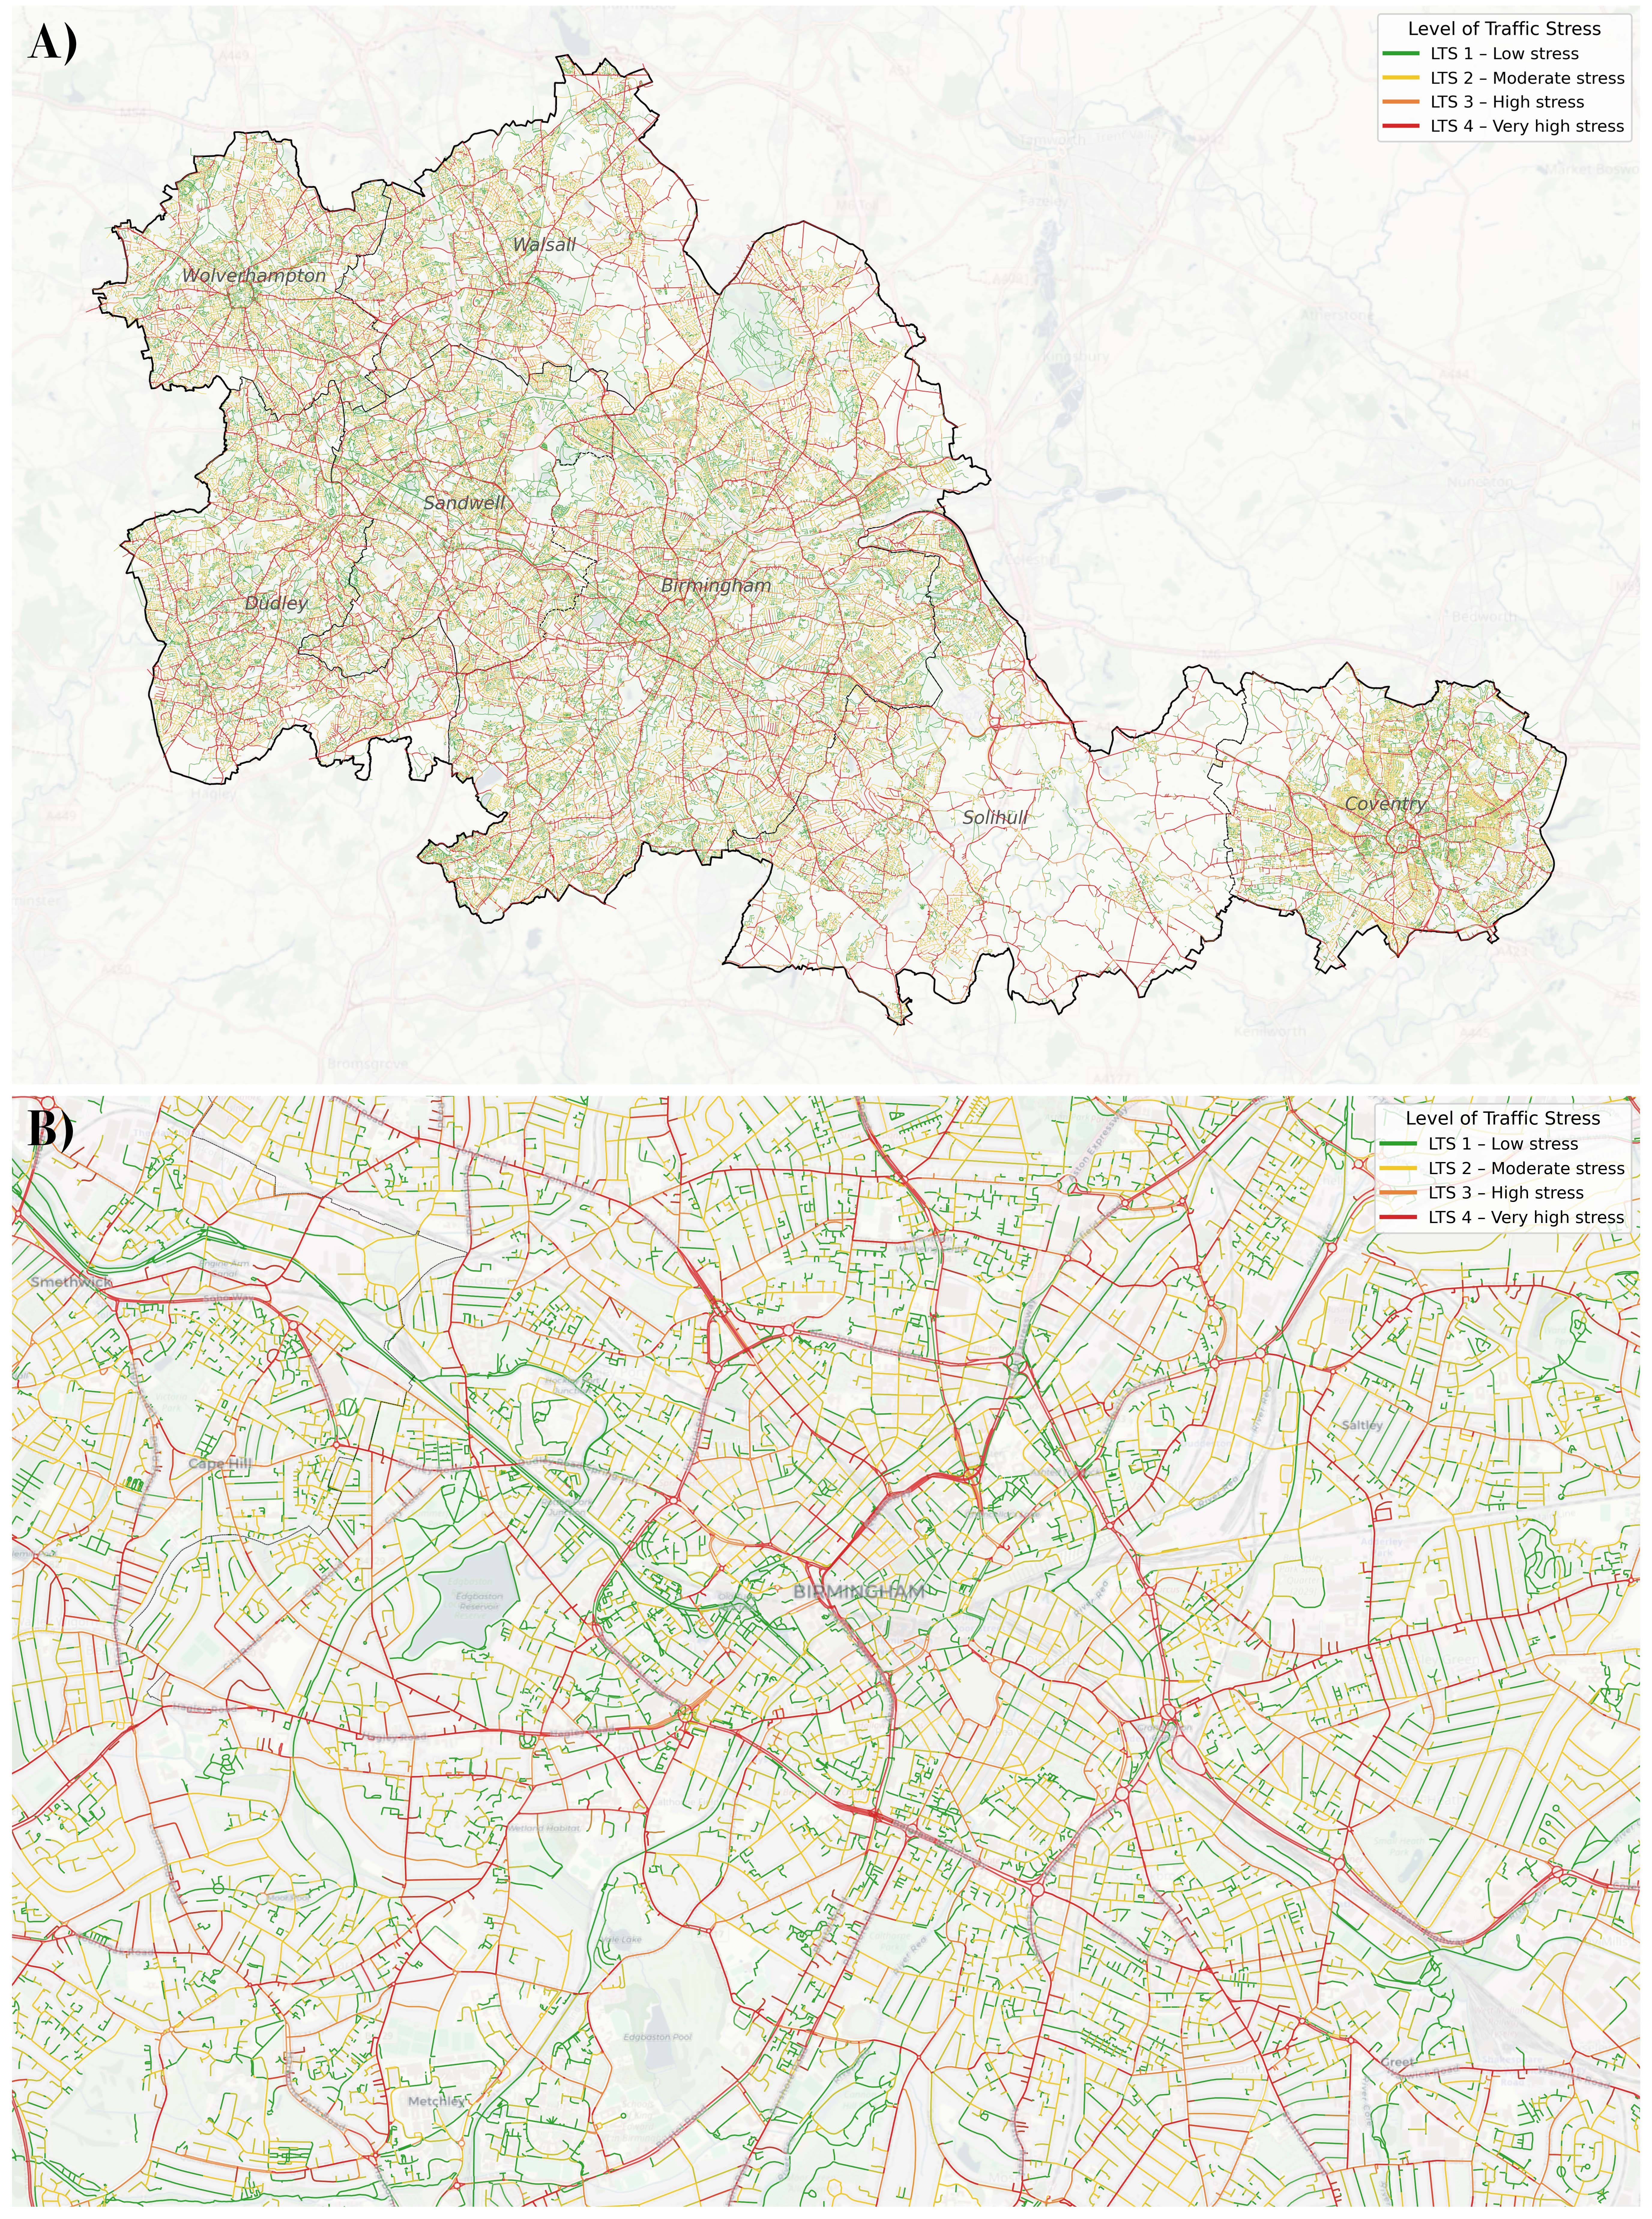
\includegraphics[width=0.8\textwidth]{figure/wm_lts.jpg}
    \caption{Final Level of Traffic Stress classification after junction stress enhancement. Where a link's two directed edges disagree, the higher value is shown.}
    \label{fig:lts-map}
\end{figure*}

\begin{figure*}[!t]
    \centering
    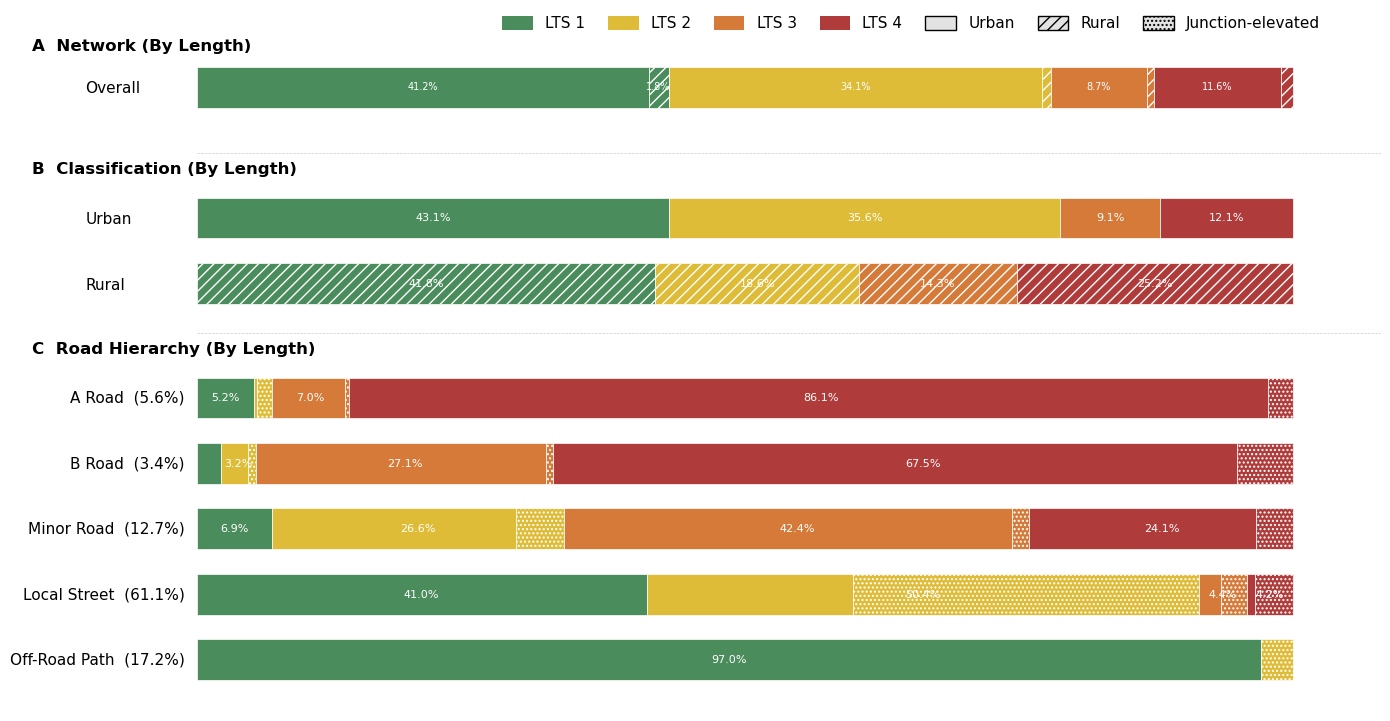
\includegraphics[width=0.8\textwidth]{figure/lts_profile.png}
    \caption{LTS distribution across the directed cyclable network.}
    \label{fig:lts_composition}
\end{figure*}

Junction stress substantially reshapes this profile: the LTS~1 share falls from 67.7\% to 47.4\% of edges, with 103,447 edges totalling 5,834~km (25.0\% of network length) elevated. Uncontrolled crossings account for most elevations (97,055 edges), with roundabout approaches contributing a further 5,123, typically to LTS~3 or~4, consistent with evidence that multi-arm roundabouts are among the most stressful cycling environments in the UK road network \citep{davies1997,reid2011}. Local Streets dominate the effect: 4,490~km of Local Street length is elevated from LTS~1 to LTS~2 at junctions, 77.0\% of all junction-elevated length.

\subsection{Stress-based Network Density and Fragmentation}
\label{sec:density}

Across 1,718 LSOAs, LTS~1 and LTS~2 record median absolute densities of 13.9 and 12.3~km/km\textsuperscript{2}, far higher than LTS~3 (3.0) and LTS~4 (3.6). Relative density shows mean LTS~1 and LTS~2 shares of 41.6\% and 37.3\%, a combined low-stress mean of 78.9\%. Joining Census 2021 population, nearly two-thirds of the region's residents (64.7\%, approximately 1.89~million) live in LSOAs where low-stress segments constitute at least 75\% of local network length. This local abundance does not, however, translate into connected routes.

Table~\ref{tab:fragmentation} reports fragmentation metrics computed on the LCC of the full cyclable network (10,634.6~km). At LTS~$\leq 1$, the sub-network fragments into 26,176 connected components with a mean size of 0.19~km; its LCC spans just 181.9~km, 3.7\% of sub-network length. Relaxing to LTS~$\leq 2$ reduces the component count to 9,637, but the LCC share rises only to 6.5\% (517.5~km), confirming that the low-stress network remains severely fragmented. A qualitative transition occurs at LTS~$\leq 3$, where the LCC absorbs roughly a third of the sub-network (32.7\%) as arterial links bridge previously isolated clusters. 

Figure~\ref{fig:fragmentation} makes these patterns visible in distributional terms. The rank-size plot (Panel A) steepens markedly at lower stress levels, reflecting the compression of component sizes documented in Table~\ref{tab:fragmentation}. Panel B captures the corresponding trade-off: as the threshold relaxes, total network length increases while the component count falls. The length-weighted KDE (Panel C) translates fragmentation into the cyclist's experience: at LTS~1, the distribution peaks at 0.33~km, meaning a randomly selected low-stress segment typically belongs to a component spanning
only a few hundred metres. At LTS~$\leq$~2 the peak shifts to 9.1~km, yet most network length remains distributed across mid-size components rather than consolidated into a connected backbone.

Junctions are a critical source of this fragmentation. Incorporating junction stress increases the LTS~1 component count by 39.7\% (18,732 to 26,176) while total length contracts by 21.7\% (6,329.0 to 4,955.6~km), as high-stress crossings sever links that previously connected adjacent clusters; the LCC contracts from 311.8 to 181.9~km and mean component size halves. The effect persists at LTS~$\leq 2$, where the LCC share falls from 7.8\% to 6.5\%. The apparent abundance of low-stress infrastructure identified in Section~\ref{sec:density} does not translate into usable continuous routes.

\begin{figure*}[!t]
    \centering
    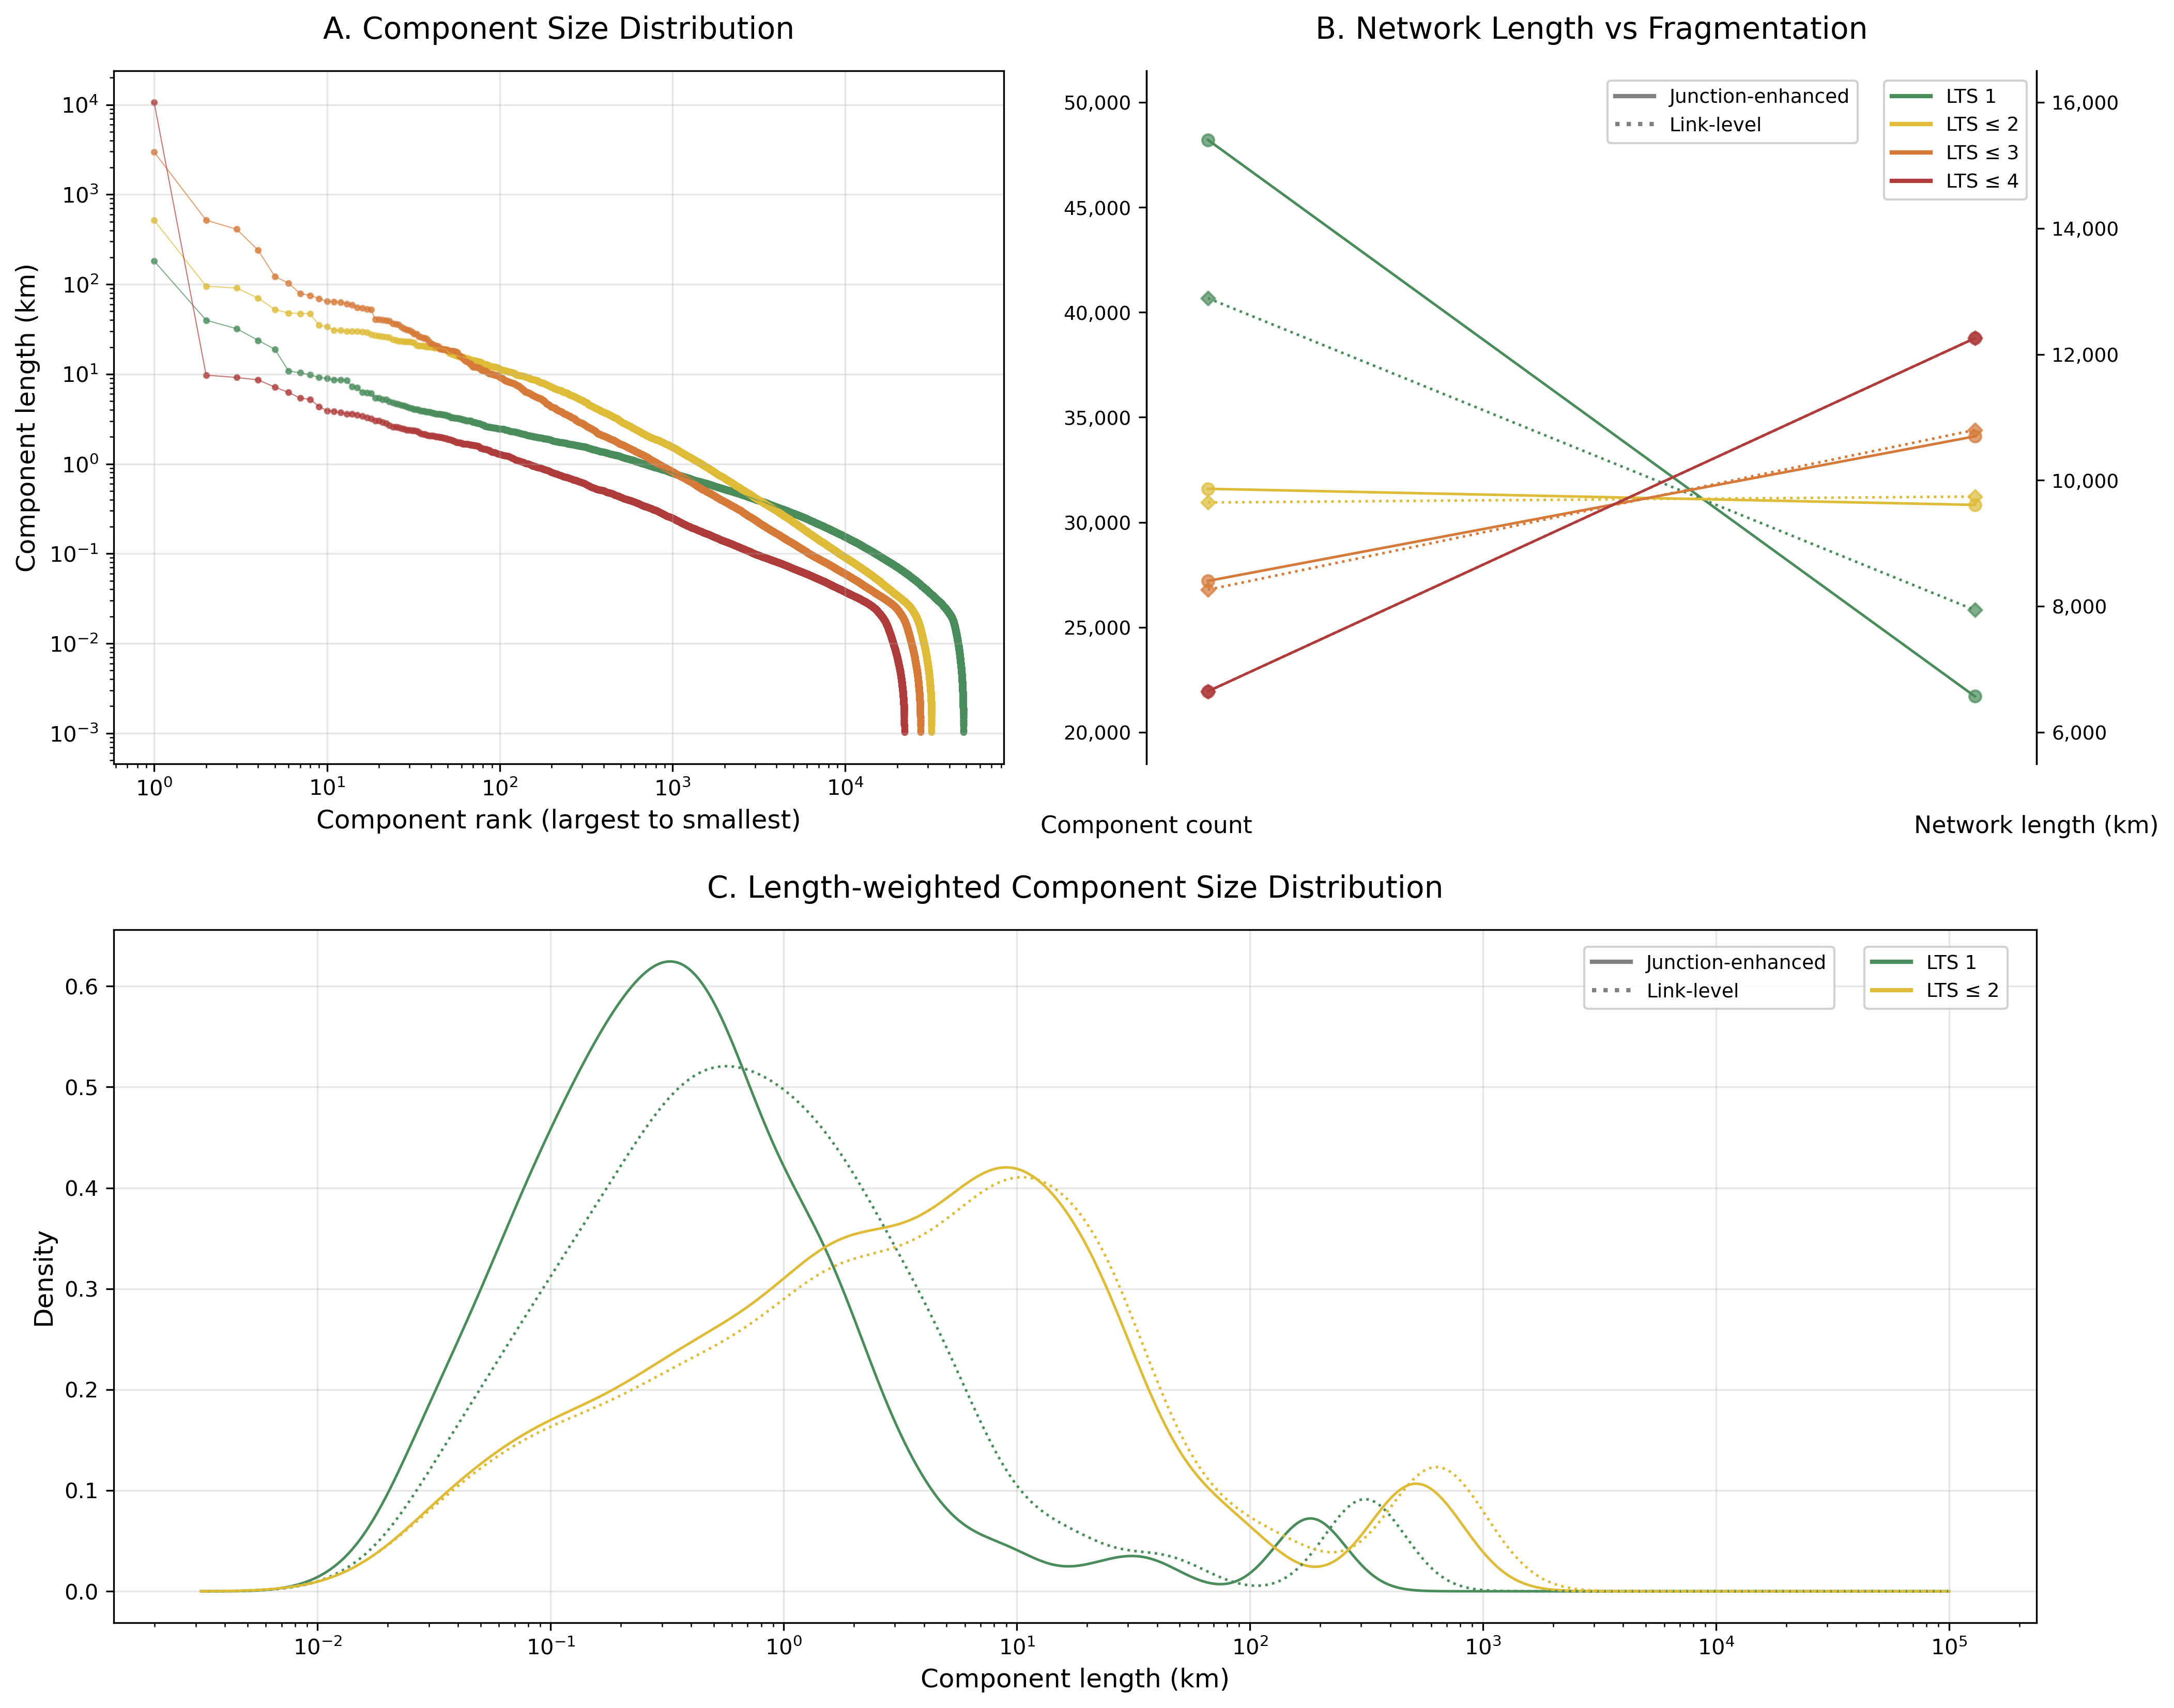
\includegraphics[width=0.78\textwidth]{figure/wm_lts_fragmentation.png}
    \caption{Fragmentation of the West Midlands cyclable network by cumulative LTS threshold.}
    \label{fig:fragmentation}
\end{figure*}

\begin{table*}[!t]
\centering
\caption{Fragmentation metrics by cumulative LTS threshold, computed on the LCC of the full cyclable network.}
\label{tab:fragmentation}
\begin{tabular}{llrrrrr}
\hline
LTS threshold & Classification & Network (km) & Components & Mean size (km) & LCC (km) & LCC share (\%) \\
\hline
$\leq 1$ & Link-level & 6,329.0 & 18,732 & 0.34 & 311.8 & 4.9 \\
         & Junction-enhanced & 4,955.6 & 26,176 & 0.19 & 181.9 & 3.7 \\
$\leq 2$ & Link-level & 8,128.2 & 8,993 & 0.90 & 634.4 & 7.8 \\
         & Junction-enhanced & 7,996.9 & 9,637 & 0.83 & 517.5 & 6.5 \\
$\leq 3$ & Link-level & 9,184.4 & 4,841 & 1.90 & 3,276.7 & 35.7 \\
         & Junction-enhanced & 9,083.4 & 5,260 & 1.73 & 2,972.6 & 32.7 \\
$\leq 4$ & Both & 10,634.6 & 1 & 10,634.6 & 10,634.6 & 100.0 \\
\hline
\end{tabular}
\end{table*}

\subsection{Network Reach and Origin-destination Connectivity}
\label{sec:reach-od}

At LTS~1, reach within 8~km is negligible: the median LSOA records just 0.1~km and 37.0\% of LSOAs have zero reach entirely (Fig.~\ref{fig:network-reach}). At LTS~$\leq 2$ the median rises to 10.6~km (mean 37.5~km), but 9.5\% of LSOAs still register zero and the distribution remains heavily right-skewed. Higher-reach LSOAs align with the few continuous off-road corridors identified in Section~\ref{sec:density}, most notably the Birmingham Canal towpath. The median reach at LTS~$\leq 2$ is just 0.7\% of that available at LTS~$\leq 4$, quantifying the connectivity penalty imposed on stress-averse cyclists.

The origin-destination analyses target the user groups central to ``cycling for all'' (Fig.~\ref{fig:od-connectivity}). Only 4.1\% of the region's population can reach their nearest school via a route within LTS~1, the threshold deemed suitable for children. LTS~1 school access is scattered across urban LSOAs with no distinct clustering, arising where schools happen to fall within short-residential or off-road segments; at LTS~$\leq 2$, school accessibility reaches 65.4\%, still leaving over a third of the population without a low-stress school route. Of inter-MSOA commuting pairs within 8~km straight-line distance, only 13.0\% of flow is connected at LTS~$\leq 2$, and connected pairs face a median detour of 1.76 times the unconstrained shortest path (flow-weighted mean 2.46). Connectivity is highest around the off-road corridors of Sandwell, Dudley and western Birmingham, and near zero across southern Birmingham, Solihull and Coventry. A qualitative transition occurs at LTS~$\leq 3$, where 50.8\% of flow becomes connected with a median detour of 1.49. These results indicate the network fails to deliver adequate low-stress connectivity for either school trips or commutes, and where routes exist, low-stress routing roughly doubles journey distance.

\begin{figure*}[p]
    \centering
    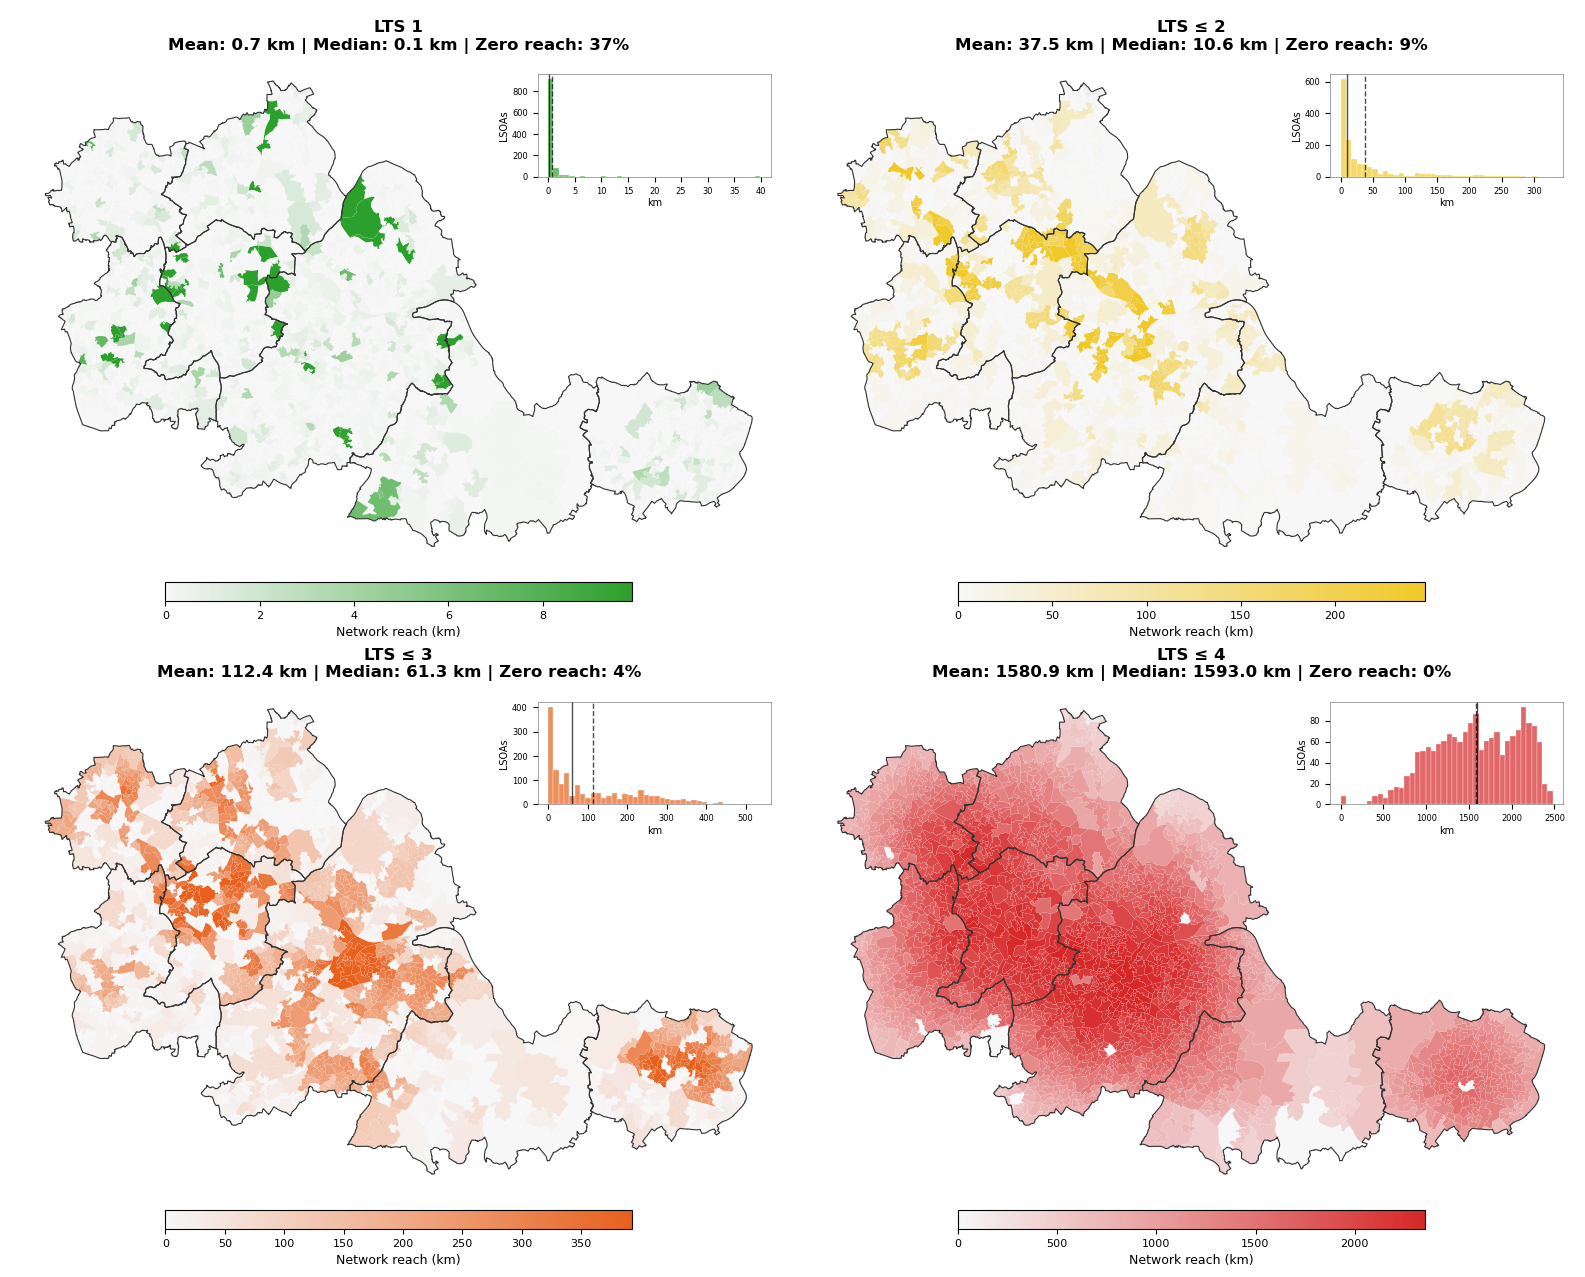
\includegraphics[height=0.46\textheight,keepaspectratio]{figure/network_reach.png}
    \caption{Network reach within 8~km from each LSOA centroid at four cumulative
    LTS thresholds.}
    \label{fig:network-reach}

    \vfill

    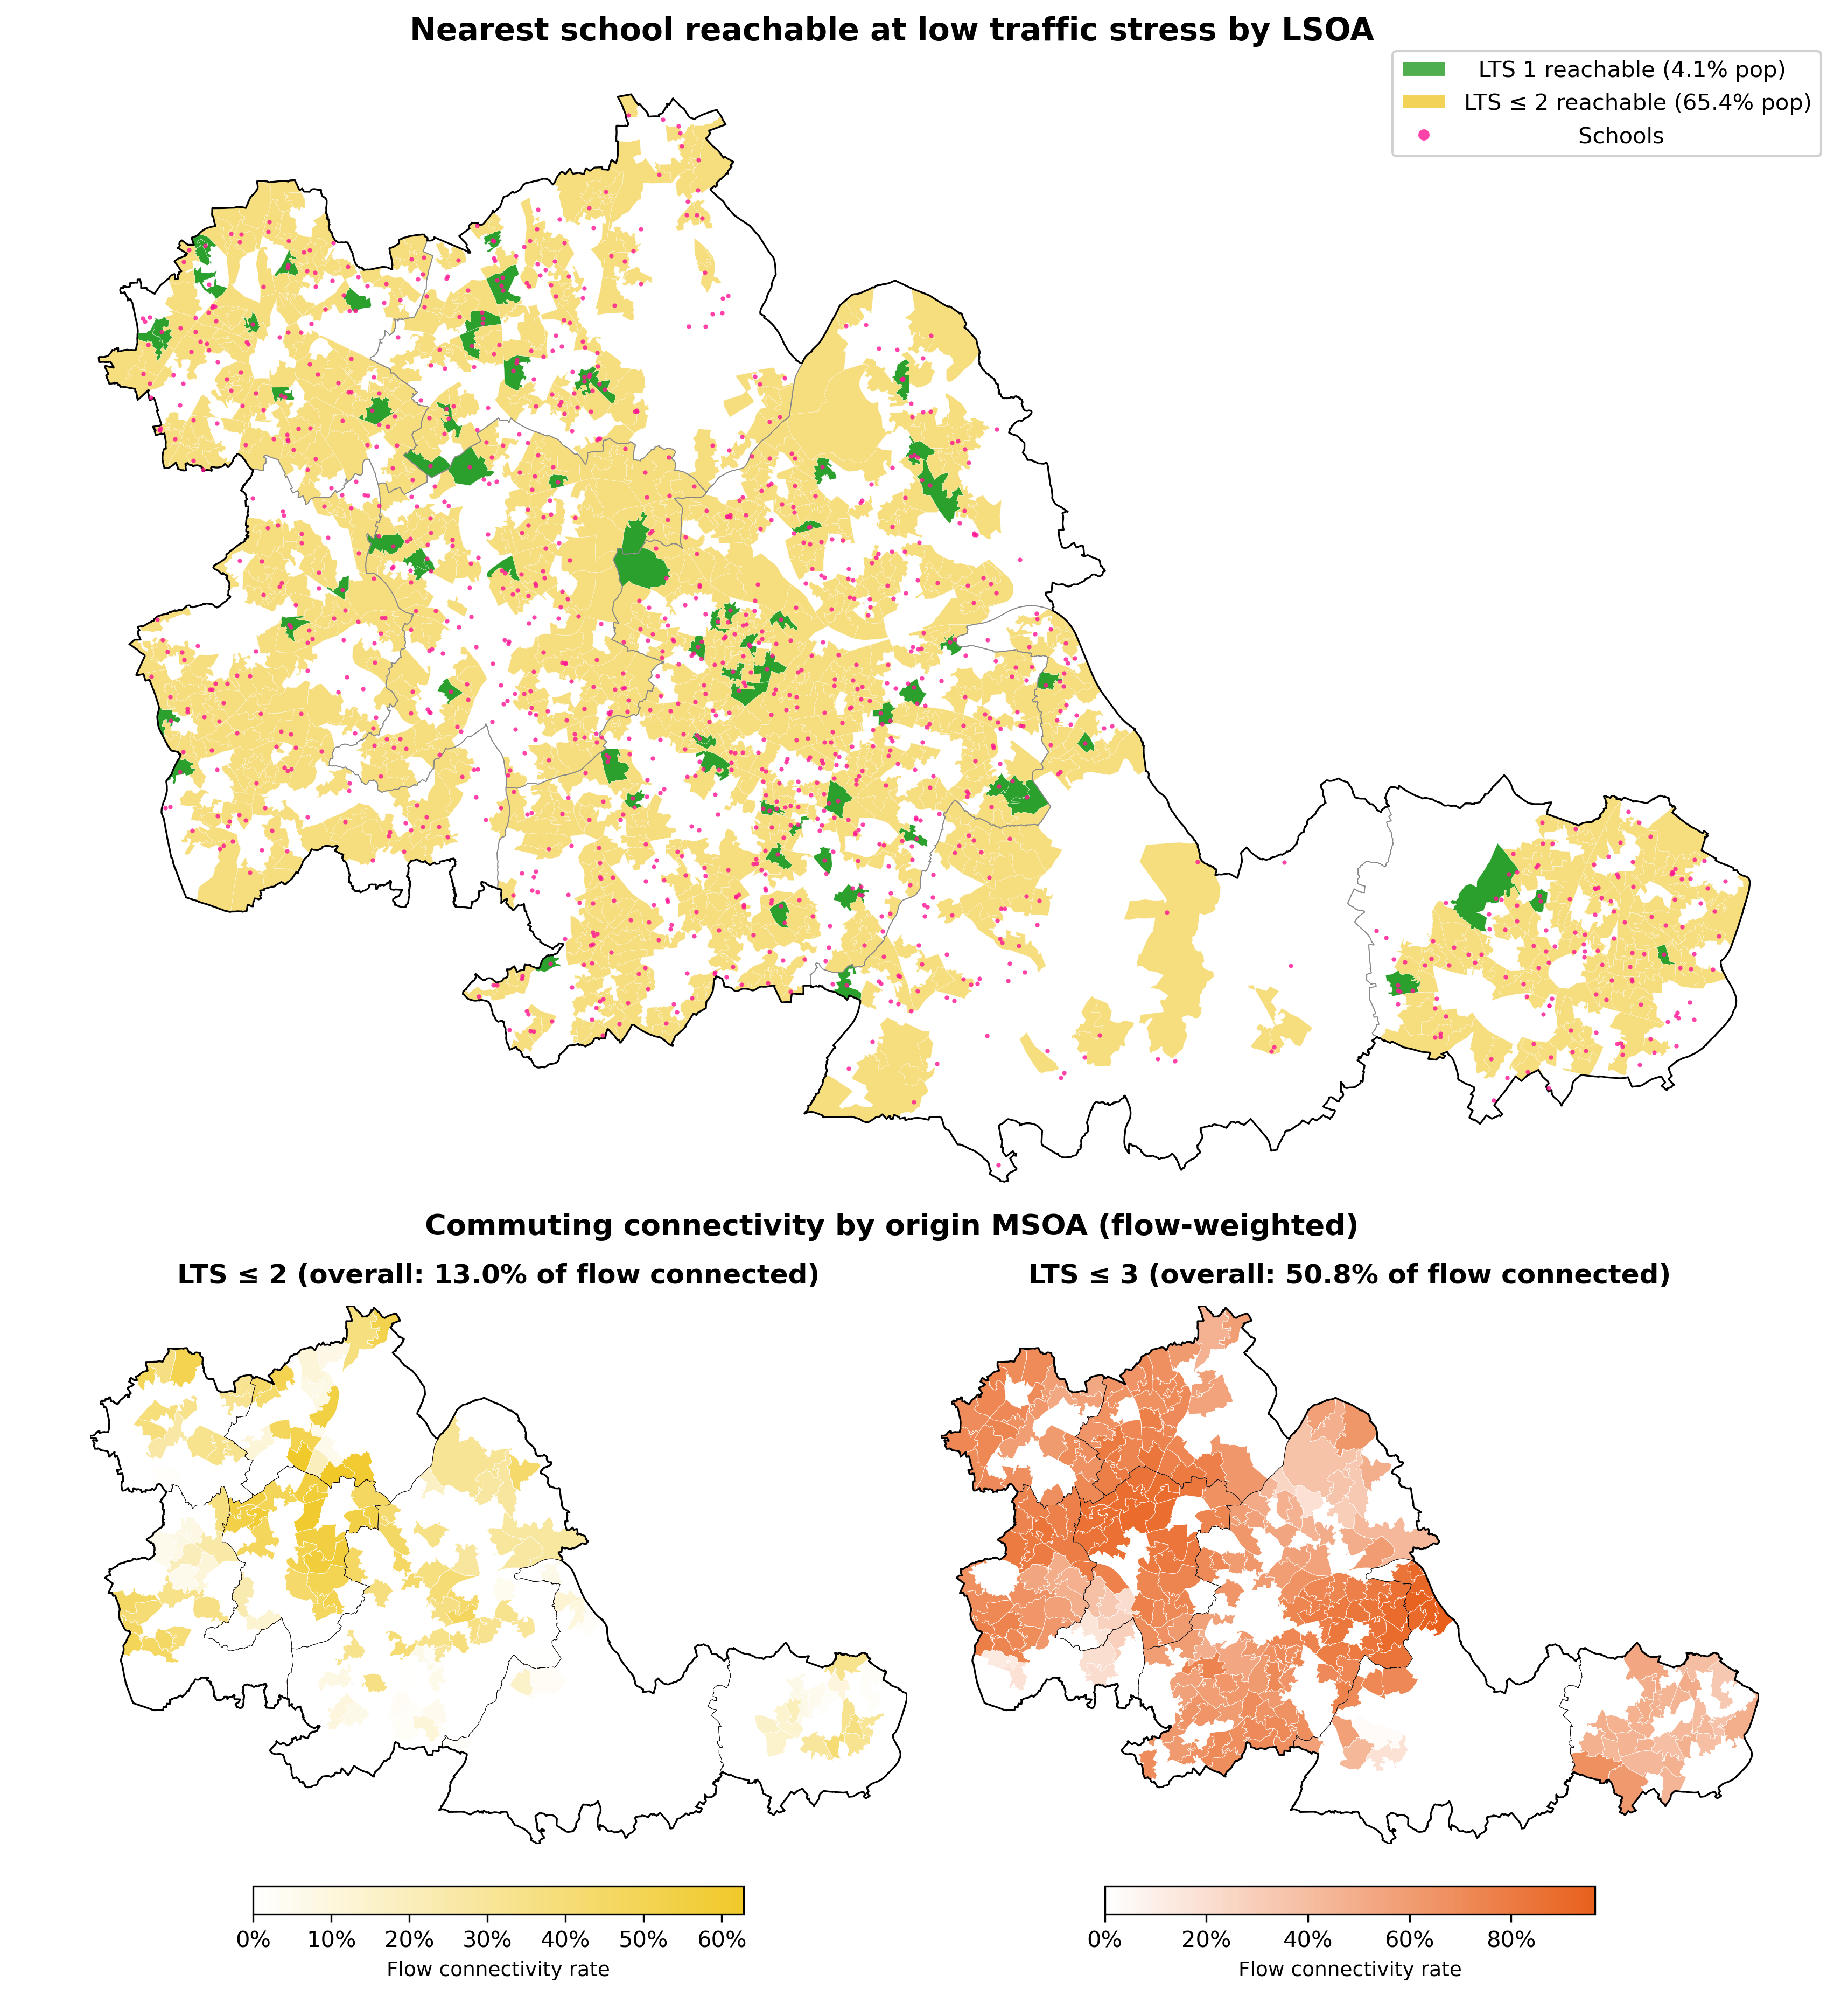
\includegraphics[height=0.46\textheight,keepaspectratio]{figure/od_connectivity_combined.png}
    \caption{Destination connectivity at low traffic stress.}
    \label{fig:od-connectivity}
\end{figure*}

\section{Discussion}
\label{sec:discussion}

\subsection{Evaluating ``Cycling for All'': Network Connectivity Against LTN 1/20}
\label{sec:disc-cycling-for-all}

Because the classification is drawn directly from LTN~1/20's own criteria, the connectivity indicators are not judgements imposed by an external standard but the standard measuring itself. By that measure the West Midlands falls far short: low-stress reach contracts so severely that the network accessible to stress-averse cyclists is negligible relative to the full cyclable network, leaving most short-distance commuting demand, the component of travel most spatially regular and therefore most amenable to infrastructure-led mode shift, either unconnectable at tolerable stress levels or viable only through detours that eliminate cycling's competitive advantage over driving. These findings are consistent with observed behaviour. The region's 0.9\% cycling mode share sits within a national picture essentially unchanged since 2002 \citep{departmentfortransport2025}, and \citet{cervero2019}, modelling cycle commuting across 36 British cities and towns, found the diversion penalty between low-stress and shortest paths to be a significant negative predictor of mode share, with each 10-percentage-point increase in very-low-stress links corresponding to a 0.65-point increase in cycling. Rather than indicating purely cultural car dependence, the results suggest that network structure is at minimum consistent with, and plausibly contributes to, the region's low cycling uptake.

\subsection{Junction Stress as the Network Expression of Arterial Severance}
\label{sec:disc-junction}

The Conveyal-lineage approach that dominates applied LTS practice assigns the
highest segment LTS at a vertex to all incident edges, without distinguishing
travel direction or crossing conditions. The directed classification developed
here propagates stress only to edges whose cyclist confronts conflicting
traffic, and applies roundabout-specific criteria that existing implementations
lack. In a network where physically separated on-carriageway provision is
minimal, these design-guidance-consistent criteria make visible how arterial
traffic conditions propagate through junctions to sever the low-stress network.

Junction stress, whether through the incremental erosion of crossing or the
near-absolute severance of roundabouts, reclassifies a modest share of total
network length yet fragments the low-stress network far beyond that proportion.
This reflects the network's own structure: low-stress segments form short
residential clusters (predominantly Local Streets) connected through a small
number of nodes where they meet higher-classification roads, and these nodes are
precisely where the speed and volume of crossing traffic trigger junction
stress. The effect concentrates at the topological bottlenecks between clusters,
severing connections that cannot be replaced by alternative routes. Junction
stress is thus best understood as the network expression of arterial severance
rather than a consequence of junction form alone: arterials impose high stress
along their links, and junctions extend that stress into the residential streets
that must cross them, a dimension that link-level classification would miss and
Conveyal-lineage approach would overstate.

\subsection{Assessing OS NGD Cycle Lane Data: A First Independent Comparison with OSM}
\label{sec:disc-osngd}

OSM is increasingly central to cycling infrastructure research, in the UK as elsewhere \citep{ferster2020, lovelace2020, nelson2021}, but its decentralised contribution model produces known tagging inconsistencies, and attributes such as lane width and directionality are absent or inconsistently recorded \citep{wasserman2019, lukawska2026}. The OS~NGD Cycle Lane collection offers an authoritative alternative with a uniform national capture specification, yet its completeness, on which all downstream LTS results depend, has not previously been independently assessed. Comparison against OSM-derived infrastructure for Birmingham reveals a category-specific pattern. For physically separated infrastructure, OS~NGD records 66.3~km against 57.2~km in OSM (ratio 1.16), while distinguishing kerbed, stepped and lightly segregated tracks where OSM cannot differentiate beyond a single track category. For paint-only lanes the pattern reverses: OS~NGD records 25.5~km against 71.5~km (ratio 0.36), capturing barely one third of OSM's provision. The divergence is consistent with OS's documented aerial capture methodology \citep{ordnancesurvey2025}: kerbs and barriers produce clear aerial signatures, painted markings do not, and OSM's advantage reflects street-level contributor knowledge that an aerial survey systematically misses. The gap has limited implications for the LTS results, as paint-only lanes offer no physical protection and share near-identical classification boundaries with mixed traffic under the thresholds of Section~\ref{sec:link-lts}, and it may diminish as maintenance cycles refine the dataset. Despite the undercounting, OS~NGD Transport can support rigorous, policy-aligned network analysis, and UK cycling research stands to benefit from its adoption as coverage matures.

\subsection{Limitations and Future Work}
\label{sec:disc-limitations}
Three limitations bear on the classification. First, LTN~1/20 specifies HGV composition thresholds alongside AADT, reflecting HGVs' disproportionate involvement in cyclist fatalities \citep{morgan2010, chao2025}; network-wide composition data were unavailable, potentially underestimating stress on high-freight routes. Second, $V_{85}$ estimation applies a fixed multiplier assuming a normal speed distribution, which may misrepresent prevailing speeds where traffic calming or congestion skews distributions. Third, the primal-graph junction representation assigns the same stress to all turning movements from an approach edge, whereas a right turn involving no crossing and a through movement across a high-stress leg carry very different stress; \citet{furth2026}, led by the original author of the LTS framework, address this through a dual-graph representation with movement-level stress values, and integrating it with the LTN~1/20-grounded classification is a direction for future work. More fundamentally, the classification inherits LTN~1/20's design thresholds; while each threshold draws on specific safety evidence, their combination into a unified stress classification has not been validated against cyclist-perceived stress. Stated-preference surveys, revealed route choice or GPS trajectory analysis could test this correspondence, evaluating the underlying standard rather than this operationalisation.

%% ============================================================

\section{Conclusion}
\label{sec:conclusion}
This paper set out to address the absence of a data-driven,
network-level methodology for evaluating cycling infrastructure quality in
England. While LTN~1/20 established the most comprehensive national design
standards to date, its evaluation instruments were conceived for scheme-level
auditing and cannot assess whether a city's network, taken as a whole, delivers
the connected low-stress conditions that its ``cycling for all'' principle
requires. In response, this study developed a directed Level of Traffic Stress
classification grounded entirely in LTN~1/20's own criteria and applied it to
the West Midlands using the newly released OS NGD Transport data.

The contributions of this study span methodology and data. Methodologically,
the classification replaces North American LTS thresholds with those derived
from the CLoS Safety subcriteria, the JAT and the design criteria, producing the
first LTS framework calibrated to English design standards and thereby restoring
the population-anchored logic that LTN~1/20's compensatory scoring obscures. The
directed network representation and bearing-based junction assessment further
extend LTS practice beyond undirected max-propagation, incorporating
roundabout-specific criteria absent from all prior implementations. Beyond
methodology, the study provides the first independent assessment of the OS NGD
Cycle Lane dataset, establishing both its strengths in recording separated
infrastructure and its systematic undercapture of paint-only provision, an
evaluation that conditions the reliability of any future research built on this
data source.

The findings demonstrate that abundant low-stress length does not constitute a
usable network. Although low-stress segments dominate the West Midlands network
by length, they fragment into ten thousands of disconnected components.
Arterial roads emerge as the primary source of severance, imposing high stress
both along their links and at the junctions where residential clusters must
cross them, with roundabouts functioning as near-absolute points of severance;
reach at tolerable stress collapses to the immediate residential cluster,
terminating where the first arterial crossing is encountered. The consequence is
that neither children nor mainstream adults can rely on the network for everyday
journeys: only 4.1\% of residents can reach their nearest school under conditions
suitable for children, and only 13.0\% of short-distance commuting flow is
connected at levels tolerable to mainstream adults, with connected journeys
requiring substantial detours.

Because both the classification thresholds and the underlying data are national
in scope, the framework can be applied to any English city without
recalibration, enabling systematic benchmarking of network conditions against a
single statutory standard. By translating LTN~1/20's design criteria into a
stress classification, the standard can be turned back on the networks it
governs, revealing in quantitative terms the distance between the ambition of
cycling for all and the infrastructure through which that ambition must be
realised.

\section*{Data availability}

Road network data from the Ordnance Survey National Geographic Database (OS~NGD) Transport theme were provided by Transport for West Midlands as part of a research collaboration. OS~NGD is a commercially licensed product available from Ordnance Survey; UK academic institutions can access equivalent data through EDINA Digimap. Derived network classification outputs and analysis code are available at \url{https://zhengpei-xu.github.io/CASA/CASA0004_Dissertation/docs/}.

\section*{Declaration of competing interest}

The author declares thats he has no known competing financial interests or personal relationships that could have appeared to influence the work reported in this paper.

%% ============================================================
\bibliographystyle{elsarticle-harv}
\bibliography{references}

\end{document}


